\section{Opgave 1}
\subsection{Beskrivelse og Design}
	Et program ønskes, der kan omskrive arabiske tal til romerske,
	således at ex. 15 konverteres til \emph{XV}.
	
	Romertal er opbygget af en række bogstaver med forskellige værdier,
	\emph{I} har værdien 1 \emph{V}, værdien 5. En komplet liste over værdier findes i tabel~\ref{fig:romertal1}.
	Det ses at nogle værdier kan udtrykkes på flere måder, en liste over vores valg af bogstaver findes i tabel~\ref{fig:romertal2}.
	
	Romertal stykkes så sammen af disse bogstaver, læses de fra højre mod venstre lægges værdierne af de bogstaver man møder sammen;
	med mindre man møder et bogstav, med en værdi mindre end de forgående. I dette tilfælde trækkes værdien fra.
	Det er kun ``lovligt'' at trække ét bogstav fra af gangen og kun hvis dette har en værdi der ligger en dekade under værdien af det forgående bogstav.
	Desuden skal det være et bogstav med værdien $10^n~n\in\mathbb{N}$.
	Dvs. der må stå et enkelt \emph{I} før \emph{X} og \emph{V}, \emph{X} før \emph{C} og \emph{L} osv.
	
	I table~\ref{fig:romertal1} kan vi se at tallede 1 og 5 findes i alle dekader (op til et maksimum på 100.000.000).
	tallene 1-9 kan således skrives:
	\begin{align*}
		1 &= 1\\
		2 &= 1 + 1\\
		3 &= 1 + 1 + 1\\
		4 &= 5 - 1\\
		5 &= 5\\
		6 &= 5 + 1\\
		7 &= 5 + 1 + 1\\
		8 &= 5 + 1 + 1 + 1\\
		9 &= 10 - 1\\
	\end{align*}
	
	vælger vi bogstaver i den rigtige dekade kan vi således skrive alle cifre i tallet op til 100.000.000.
	Efter dette skiftes til 1-talssystemet, så der bare lægges det korrekte multipum af 100.000.000 til.
	
	Et flowdiagram over programmets struktur er vist i figur~\ref{fig:1a01}
	
	\begin{figure}[h!]
	  \centering
	      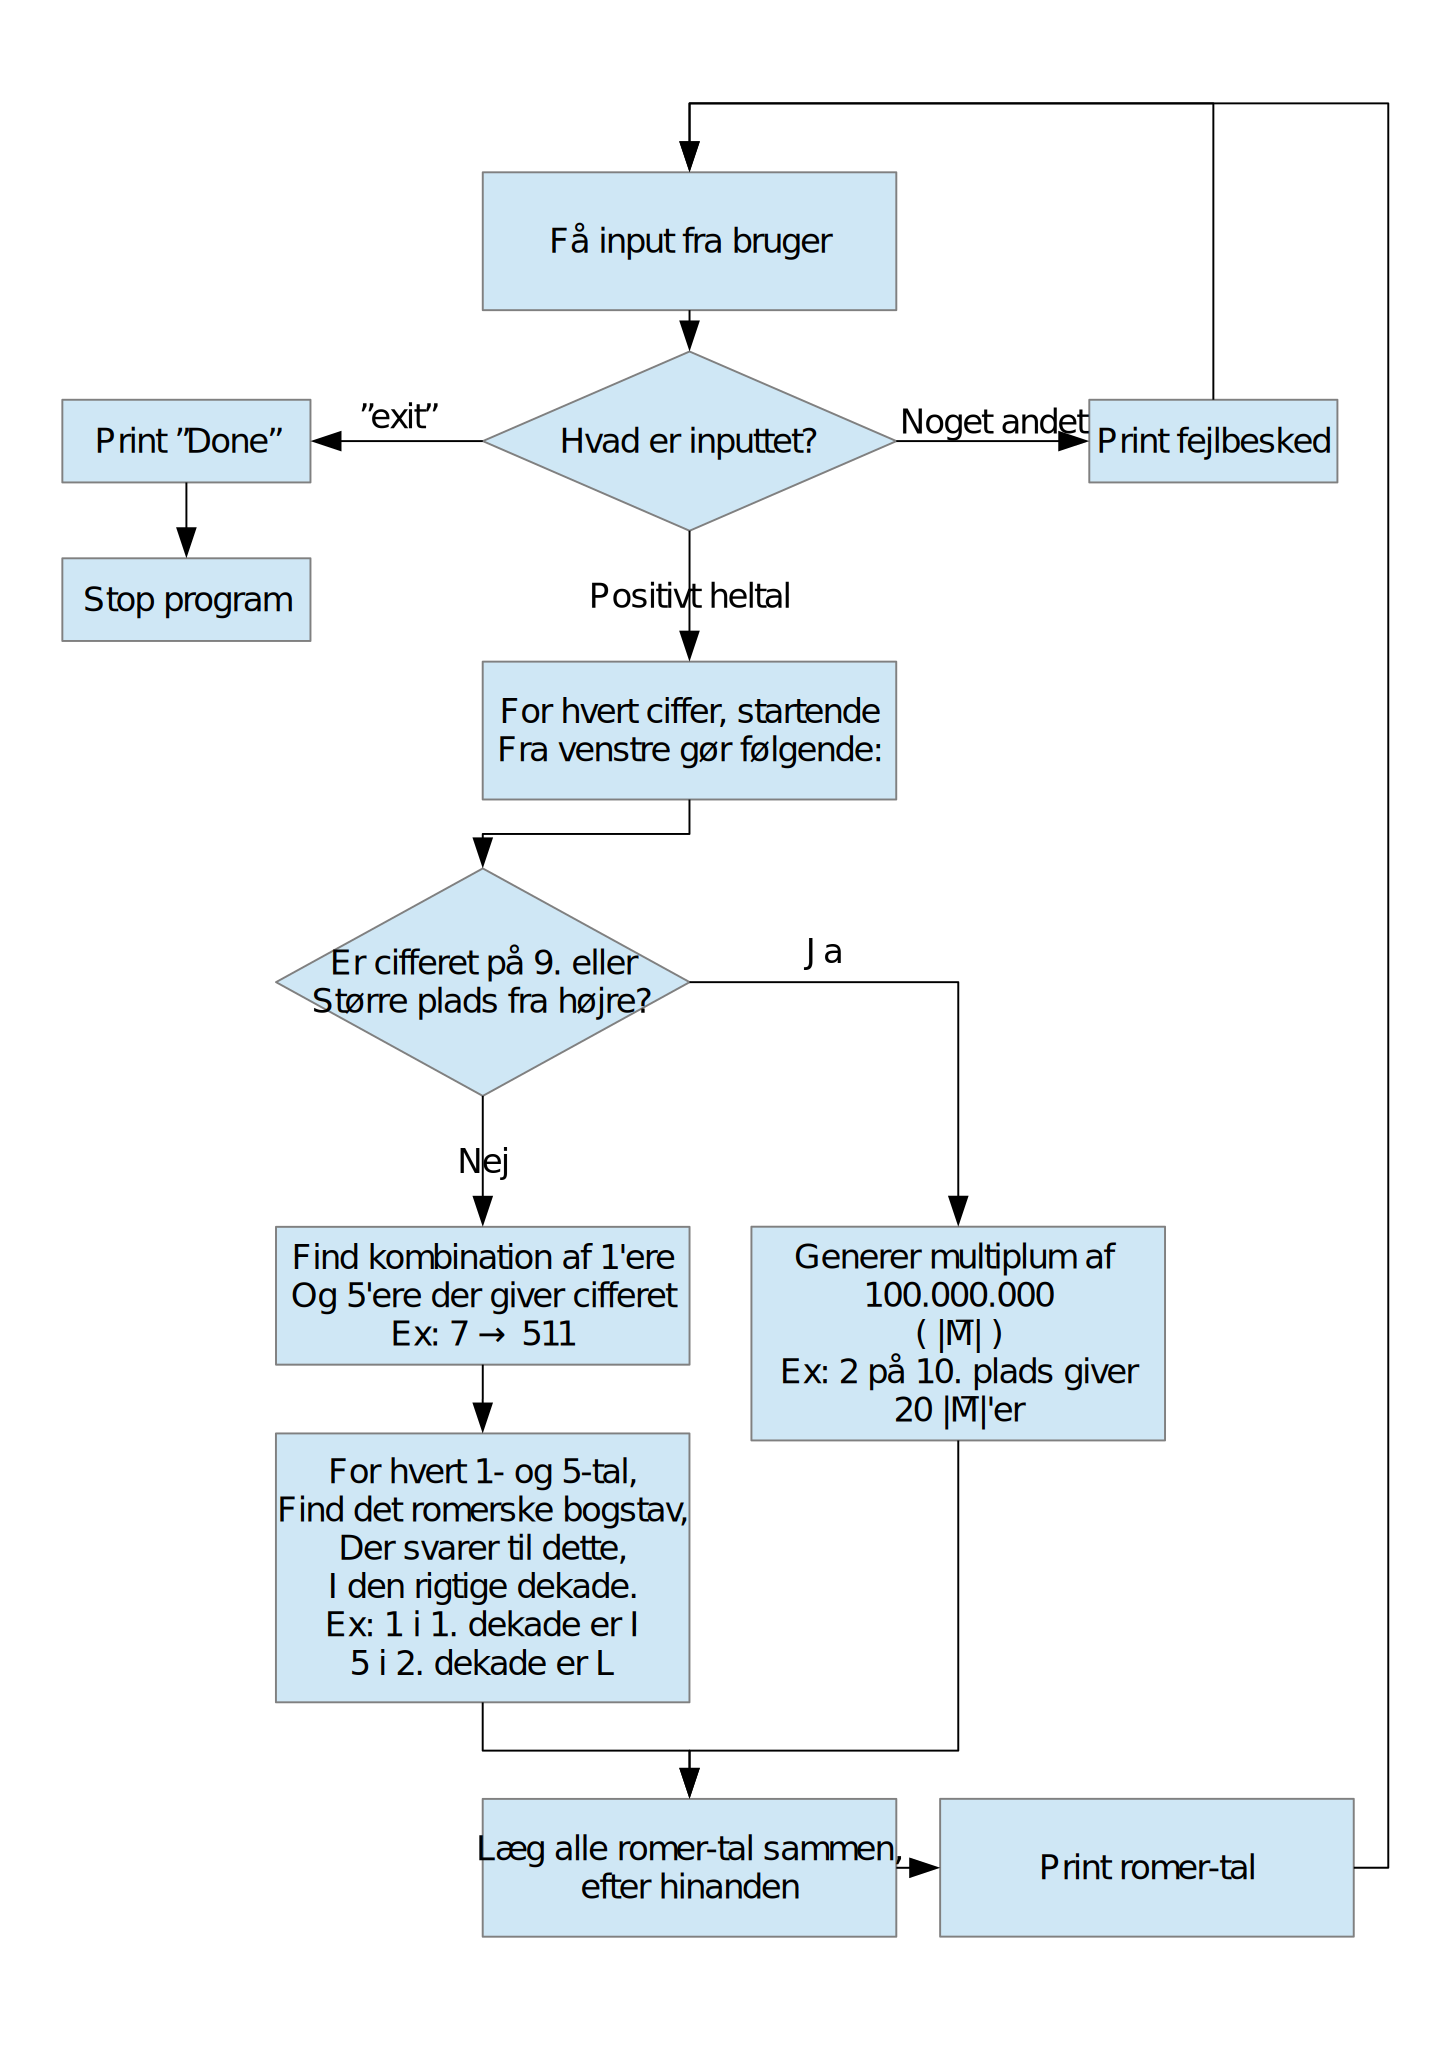
\includegraphics[width=0.8\textwidth]{1a01}
	  \caption{Flow diagram over programmets struktur}\label{fig:1a01}
	\end{figure}
		 
	\begin{table}[h!]
\begin{center}
\begin{tabular}{ | r  l || r  l | }
  \hline                        
  Værdi & bogstav & Værdi & Bogstav \\
  \hline
  1			& $I$ 								& 5				& $V$ \\
  10		& $X$ 								& 50			& $L$ \\
  100		& $C$ 								& 500			& $D$ \\
  1.000		& $M,~\overline{I}$ 				& 5.000			& $\overline{V}$ \\
  10.000	& $\overline{X}$ 					& 50.000		& $\overline{L}$ \\
  100.000	& $\overline{C},~|\overline{I}|$ 	& 500.000		& $\overline{D},~|\overline{V}|$ \\
  1.000.000	& $\overline{M},~|\overline{X}|$ 	& 5.000.000		& $|\overline{L}|$ \\
  10.000.000& $|\overline{C}|$				 	& 50.000.000		& $|\overline{D}|$ \\
  100.000.000& $|\overline{M}|$ & &\\
  \hline  
\end{tabular}
\caption{Romertal og deres værdier}\label{fig:romertal1}
\end{center}
\end{table}

\begin{table}[h!]
\begin{center}
\begin{tabular}{ | r  l || r  l | }
  \hline                        
  Værdi & bogstav & Værdi & Bogstav \\
  \hline
  1			& $I$ 				& 5				& $V$ \\
  10		& $X$ 				& 50			& $L$ \\
  100		& $C$ 				& 500			& $D$ \\
  1.000		& $M$ 				& 5.000			& $\overline{V}$ \\
  10.000	& $\overline{X}$ 	& 50.000		& $\overline{L}$ \\
  100.000	& $|\overline{I}|$ 	& 500.000		& $|\overline{V}|$ \\
  1.000.000	& $|\overline{X}|$ 	& 5.000.000		& $|\overline{L}|$ \\
  10.000.000& $|\overline{C}|$	& 50.000.000		& $|\overline{D}|$ \\
  100.000.000& $|\overline{M}|$ & &\\
  \hline  
\end{tabular}
\caption{Vores valg af romertal}\label{fig:romertal2}
\end{center}
\end{table}



\subsection{Programtest}
	For at teste at dette program virker som forventet er det nødvendigt at teste følgene:
 	\begin{enumerate}
 		\item Programmet håndterer hver dekade korrekt og lægger dekader korrekt sammen
 		\item Programmet håndterer fejl-input uden at bryde sammen og at det genkender exit kommandoen
 	\end{enumerate}
 	For at teste at programmet håndterer hver dekade op til 100.000.000 som er den højeste dekade programmet har et romersk numeral for, er der inkluderet en metode kaldet $testDecades$ i klassen $RomanNumerals$ som tilgås ved at indtaste den skjulte kommando "test" i konsollen. Resultatet af dette ses nedenfor:
	\begin{lstlisting}[caption=output fra kørsel af testDecades]
Input any positive integer. Type "exit" to end the program
test
STARTING TEST
1*10^1 = X  2*10^1 = XX  3*10^1 = XXX  4*10^1 = XL  5*10^1 = L  6*10^1 = LX  7*10^1 = LXX  8*10^1 = LXXX  9*10^1 = XC  
1*10^2 = C  2*10^2 = CC  3*10^2 = CCC  4*10^2 = CD  5*10^2 = D  6*10^2 = DC  7*10^2 = DCC  8*10^2 = DCCC  9*10^2 = CM  
1*10^3 = M  2*10^3 = MM  3*10^3 = MMM  4*10^3 = MV̅  5*10^3 = V̅  6*10^3 = V̅M  7*10^3 = V̅MM  8*10^3 = V̅MMM  9*10^3 = MX̅  
1*10^4 = X̅  2*10^4 = X̅X̅  3*10^4 = X̅X̅X̅  4*10^4 = X̅L̅  5*10^4 = L̅  6*10^4 = L̅X̅  7*10^4 = L̅X̅X̅  8*10^4 = L̅X̅X̅X̅  9*10^4 = X̅C̅  
1*10^5 = C̅  2*10^5 = C̅C̅  3*10^5 = C̅C̅C̅  4*10^5 = C̅|V̅|  5*10^5 = |V̅|  6*10^5 = |V̅|C̅  7*10^5 = |V̅|C̅C̅  8*10^5 = |V̅|C̅C̅C̅  9*10^5 = C̅|X̅|  
1*10^6 = |X̅|  2*10^6 = |X̅||X̅|  3*10^6 = |X̅||X̅||X̅|  4*10^6 = |X̅||L̅|  5*10^6 = |L̅|  6*10^6 = |L̅||X̅|  7*10^6 = |L̅||X̅||X̅|  8*10^6 = |L̅||X̅||X̅||X̅|  9*10^6 = |X̅||C̅|  
1*10^7 = |C̅|  2*10^7 = |C̅||C̅|  3*10^7 = |C̅||C̅||C̅|  4*10^7 = |C̅||D̅|  5*10^7 = |D̅|  6*10^7 = |D̅||C̅|  7*10^7 = |D̅||C̅||C̅|  8*10^7 = |D̅||C̅||C̅||C̅|  9*10^7 = |C̅||M̅|  
1*10^8 = |M̅|  
	\end{lstlisting}
	Herefter testes om programmet kan kombinere tal i flere dekader. Resultatet af testen ses nedenfor.
	\begin{lstlisting}[caption=Test af dekadekombination]
Input any positive integer. Type "exit" to end the program
1337
MCCCXXXVII
|M̅|
	\end{lstlisting}
	Hvilket er korrekt. \\
	\\
	Til sidst testes punkt nr. 2, at programmet afbrydes når brugeren indtaster "exit" kommandoen.
	\begin{lstlisting}[caption=Test af exit kommando]
Input any positive integer. Type "exit" to end the program
exit
Done!
	\end{lstlisting}
	Og at det kan håndtere input af negative tal samt ikke-tal.
	\begin{lstlisting}[caption=Test af dårligt input]
Input any positive integer. Type "exit" to end the program
-42
Please enter a positive integer, that's a number without a decimal point,larger than zero
Input any positive integer. Type "exit" to end the program
NaN
Please enter a positive integer, that's a number without a decimal point,larger than zero
Input any positive integer. Type "exit" to end the program
	\end{lstlisting}
	
	Disse tests opnår 100\% kode dækning. Selvom dette selvfølgelig ikke er en garanti for at programmet altid vil virke vil vi ikke gå videre med tests da det ville kræve at teste alle tænkelige input, hvilket er umuligt med den tid vi har til rådighed. Yderligere er programmet ikke begrænset af integer overflow, så dette er ikke testet.